\section{Object diffusion mini-protocol}
\label{object-diffusion-protocol}

\definecolor{mygreen}{rgb}{0.109804,0.698039,0.341176}
\definecolor{myblue}{rgb}{0.360784,0.423529,255}

\usetikzlibrary{automata, positioning, arrows}
\usetikzlibrary{arrows,calc,matrix,shapes}

\tikzset{
    state/.style={
           rectangle,
           rounded corners,
           draw=black, very thick,
           minimum height=2em,
           inner sep=2pt,
           text centered,
           },
}

\newcommand{\header}[1]{\textbf{#1}}

\newcommand{\state}[1]{\texttt{#1}}
\newcommand{\trans}[1]{\texttt{#1}}
\newcommand{\msg}[1]{\textbf{\texttt{#1}}}

\newcommand{\Client}{\textcolor{mygreen}{\textbf{Client}}}
\newcommand{\Server}{\textcolor{myblue}{\textbf{Server}}}

\newcommand{\StInit}             {\state{StInit}}
\newcommand{\StIdle}{\state{StIdle}}
\newcommand{\StBusy}{\state{StBusy}}
\newcommand{\StDone}{\state{StDone}}
\newcommand{\StObjIdsBlocking}    {\state{StObjIdsBlocking}}
\newcommand{\StObjIdsNonBlocking} {\state{StObjIdsNonBlocking}}
\newcommand{\StObjs}              {\state{StObjs}}

\newcommand{\MsgInit}            {\msg{MsgInit}}
\newcommand{\MsgRequestObjIdsNB}  {\msg{MsgRequestObjIdsNonBlocking}}
\newcommand{\MsgRequestObjIdsB}   {\msg{MsgRequestObjIdsBlocking}}
\newcommand{\MsgReplyObjIds}      {\msg{MsgReplyObjIds}}
\newcommand{\MsgRequestObjs}      {\msg{MsgRequestObjs}}
\newcommand{\MsgReplyObjs}        {\msg{MsgReplyObjs}}
\newcommand{\MsgDone}{\msg{MsgDone}}

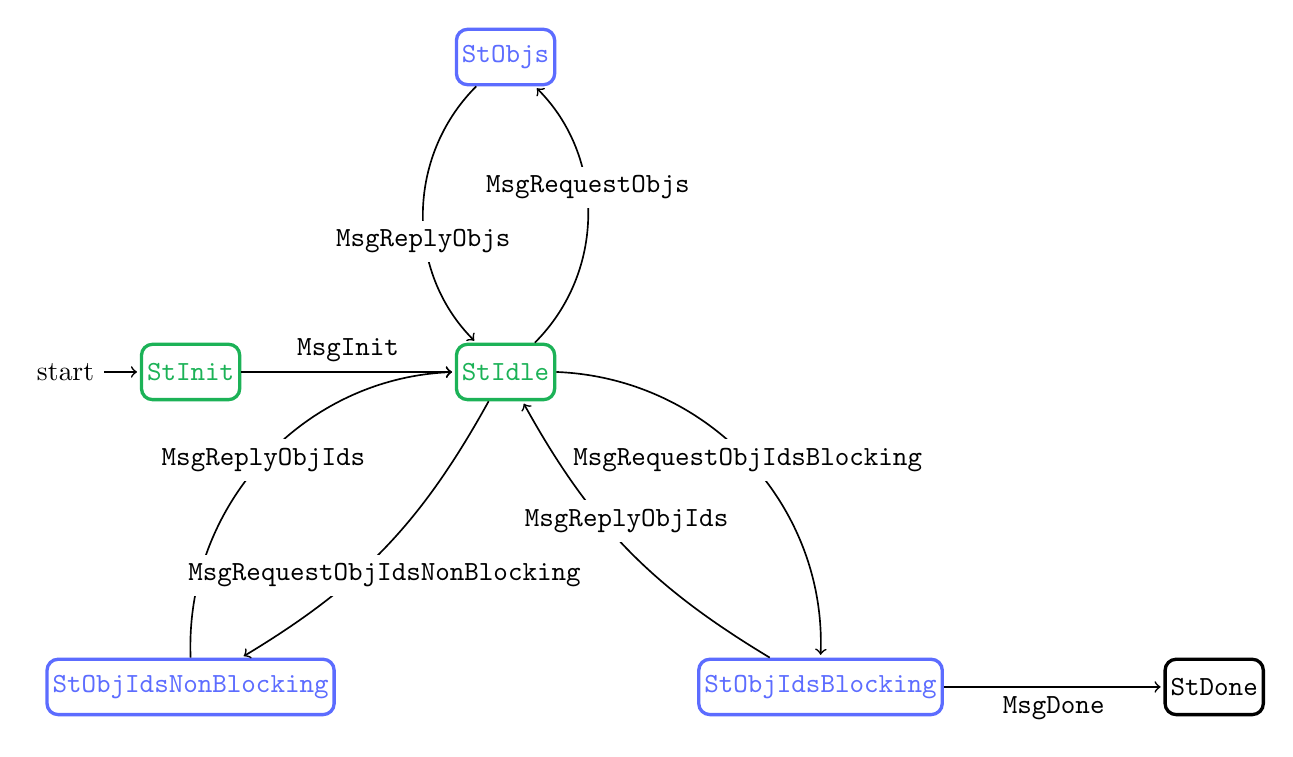
\begin{tikzpicture}[->,shorten >=1pt,auto,node distance=4.5cm, semithick]
  \tikzstyle{every state}=[fill=red,draw=none,text=white]
  \node[state, mygreen, initial] (I) at (-4,  0) {\StInit};
  \node[state, mygreen]           (A) at ( 0,  0) {\StIdle};
  \node[state]                   (B) at ( 9, -4) {\StDone};
  \node[state, myblue]          (C) at ( 4, -4) {\StObjIdsBlocking};
  \node[state, myblue]          (D) at (-4, -4) {\StObjIdsNonBlocking};
  \node[state, myblue]          (E) at ( 0,  4) {\StObjs};
  \draw (I)  edge[above]                    node[above]{\MsgInit}                                                (A);
  \draw (C)  edge[above]                    node[below]{\MsgDone}                                                (B);
  \draw (A)  edge[left, bend left=45]       node[fill = white, anchor = center]{\MsgRequestObjIdsB}               (C);
  \draw (C)  edge[right, bend left=15]      node[fill = white, anchor = center, above = 2pt]{\MsgReplyObjIds}     (A);
  \draw (D)  edge[right, bend left=45]      node[fill = white, anchor = center]{\MsgReplyObjIds}                  (A);
  \draw (A)  edge[right, bend left=15]      node[fill = white, anchor = center, below = 2pt]{\MsgRequestObjIdsNB} (D);
  \draw (A)  edge[left, bend right=45]      node[fill = white, anchor = center, above = 2pt]{\MsgRequestObjs}     (E);
  \draw (E)  edge[right,bend right=45]      node[fill = white, anchor = center, below = 2pt]{\MsgReplyObjs}       (A);
\end{tikzpicture}

\begin{figure}[h]
  \begin{center}
    \begin{tabular}{l|l}
      \header{state}       & \header{agency} \\\hline
      \StInit              & \Client \\
      \StIdle              & \Client \\
      \StObjIdsBlocking    & \Server \\
      \StObjIdsNonBlocking & \Server \\
      \StObjs              & \Server \\
    \end{tabular}
    \caption{Object diffusion state agencies}
  \end{center}
\end{figure}

\subsection{Parameters}

\newcommand\argfont[1]{\textbf{\texttt{\textit{#1}}}}

\begin{description}
\item [\argfont{object}] The abstract type of objects diffused by the protocol.
\item [\argfont{id}] Identifier that uniquely identifies an object.
\item [\argfont{objectIds}] An opaque type returned by the server when asked for object ids.
  It is not explicitely a list of $\argfont{id}$, because the server may want to add metadata to the ids,
  and/or run a compression scheme to limit the size of its response.
\item [\argfont{responseToIds}] A function with type $\argfont{objectIds} \rightarrow [\argfont{id}]$.
\item [\argfont{initialPayload}] An abstract payload that helps initialise the
  state of the server. For instance, a slot number before which the client does
  not care about the objects.
  \niols{eg. for Cert-Diffusion it would be a round number, for Vote-Diffusion it would be unit}
\end{description}

\subsection{Protocol messages}

\begin{description}
\item [\MsgInit{} {\((\argfont{initialPayload})\)}]
      Initial message of the protocol, with its payload.

\item [\MsgRequestObjIdsNB{} {$(\argfont{ack},\argfont{req})$}]
      The client asks for up to \argfont{req} new object ids and acknowledges \argfont{ack} old ids.
      The server immediately replies (possibly with an empty list).

\item [\MsgRequestObjIdsB{} {$(\argfont{ack},\argfont{req})$}]
      The client asks for up to \argfont{req} new object ids and acknowledges \argfont{ack} old ids.
      The server will block until new objects are available.

\item [\MsgReplyObjIds{} {$(\argfont{objectIds})$}]
      The server replies with the ids of its available objects.
      In the blocking case, the reply is guaranteed to contain enough information to build at least one object id with \argfont{responseToIds}.
      In the non-blocking case, the reply may not contain any actual data.

\item [\MsgRequestObjs{} {$([\argfont{id}])$}]
      The client requests objects by sending a list of object ids.
      The total size of the corresponding objects MUST not be bigger than the size limit in bytes.
      \niols{Or maybe a bit less; should we take into account the size of the boilerplate?}

\item [\MsgReplyObjs{} {$([\argfont{object}])$}]
      The server replies with the list of all the objects that were requested.
      \niols{Maybe sometimes it is not possible to derive an \argfont{id} from
        an \argfont{object}? eg. with certificates that could be just a hash? In
        those cases, wouldn't we want to return a list of pairs \((\argfont{id},
        \argfont{object})\)?}

\item [\MsgDone]
      The server terminates the mini protocol.
\end{description}

\begin{table}[h]
  \begin{tabular}{l|l|l|l}
    \header{from state}  & \header{message}    & \header{parameters}          & \header{to state}   \\\hline
    \StInit              & \MsgInit            &                              & \StIdle             \\
    \StIdle              & \MsgRequestObjIdsNB & \argfont{ack}, \argfont{req} & \StObjIdsNonBlocking \\
    \StIdle              & \MsgRequestObjIdsB  & \argfont{ack}, \argfont{req} & \StObjIdsBlocking    \\
    \StObjIdsNonBlocking & \MsgReplyObjIds     & $[(\argfont{id}, \argfont{objectMetadata})]$ & \StIdle \\
    \StObjIdsBlocking    & \MsgReplyObjIds     & $[(\argfont{id}, \argfont{objectMetadata})]$ & \StIdle \\
    \StIdle              & \MsgRequestObjs     & $[\argfont{id}]$             & \StObjs              \\
    \StObjs              & \MsgReplyObjs       & $[\argfont{object}]$         & \StIdle             \\
    \StIdle              & \MsgDone            &                              & \StDone             \\
  \end{tabular}
  \caption{Object diffusion mini-protocol messages.}
\end{table}

\subsection{Size limits per state}
\niols{FIXME}

Table~\ref{table:object-diffusion-size-limits} specifies how many bytes can be sent
in a given state; indirectly, this limits the payload size of each message.  If
a space limit is violated, the connection SHOULD be torn down.

\begin{table}[h]
  \begin{center}
    \begin{tabular}{l|r}
      \header{state}      & \header{size limit in bytes} \\\hline
      \StInit             & \texttt{5760} \\
      \StIdle             & \texttt{5760} \\
      \StObjIdsBlocking    & \texttt{2500000} \\
      \StObjIdsNonBlocking & \texttt{2500000} \\
      \StObjs              & \texttt{2500000} \\
    \end{tabular}
    \caption{size limits per state}
    \label{table:object-diffusion-size-limits}
  \end{center}
\end{table}

\subsection{Timeouts per state}
\niols{FIXME}

The table~\ref{table:object-diffusion-timeouts} specifies message timeouts in
a given state.  If a timeout is violated, the connection SHOULD be torn down.

\begin{table}[h]
  \begin{center}
    \begin{tabular}{l|r}
      \header{state}      & \header{timeout} \\\hline
      \StInit             & - \\
      \StIdle             & - \\
      \StObjIdsBlocking    & - \\
      \StObjIdsNonBlocking & \texttt{10}s \\
      \StObjs              & \texttt{10}s \\
    \end{tabular}
    \caption{timeouts per state}
    \label{table:object-diffusion-timeouts}
  \end{center}
\end{table}

\subsection{CDDL encoding specification}
\label{object-diffusion-cddl}
\niols{FIXME, but maybe it doesn't make sense at all if it is just wildly
  generalised.}

\lstset{
  xleftmargin=2pt,
  stepnumber=1,
  belowcaptionskip=\bigskipamount,
  captionpos=b,
  escapeinside={*'}{'*},
  language=haskell,
  tabsize=2,
  emphstyle={\bf},
  commentstyle=\it,
  stringstyle=\mdseries\rmfamily,
  showspaces=false,
  keywordstyle=\bfseries\rmfamily,
  columns=flexible,
  basicstyle=\small\sffamily,
  showstringspaces=false,
  morecomment=[l]\%,
}
\lstdefinelanguage{cddl}{
  morekeywords={bool,uint,nint,int,float16,float32,float64,float,bstr,bytes,tstr,text},
  morecomment=[l]{;},
  morestring=[b]",
}
\lstdefinestyle{cddl}{
  numbers=left,
  language=cddl,
  columns=fixed,
}

%% NOTE: lst imports are relative to the main file, hence the necessary
%% `protocol-changes/` prefix.
\lstinputlisting[style=cddl]{protocol-changes/object-diffusion.cddl}

\subsection{Client and server implementation}

\niols{REWRITE EVERYTHING. Client/server agency was switched, things might need
  to be generalised, hooks for eg. LoP might need to be added, ...}

The protocol has two design goals: It must diffuse transactions with high efficiency
and, at the same time, it must rule out
asymmetric resource attacks from the transaction consumer against the transaction provider.

The protocol is based on two pull-based operations.
The transaction consumer can ask for a number of transaction ids, and it can use these
transaction ids to request a batch of transactions.
The transaction consumer has flexibility in the number of transaction ids it requests,
whether to actually download the transaction body
and flexibility in how it batches the download of transactions.
The transaction consumer can also switch between requesting transaction ids and downloading
transaction bodies at any time.
It must, however, observe several constraints that are necessary for a memory-efficient implementation
of the transaction provider.

Conceptually, the provider maintains a limited size FIFO of outstanding transactions per consumer.
(The actual implementation can, of course, use the data structure that works best).
The maximum FIFO size is a protocol parameter.
The protocol guarantees that, at any time, the consumer and producer agree on the current size of
that FIFO and on the outstanding transaction ids.
The consumer can use a variety of heuristics to request transaction ids and transactions.
One possible implementation for a consumer is to maintain a FIFO that mirrors the producer's FIFO
but only contains the transaction ids (and the size of the transaction) and not the full transactions.

After the consumer requests new transaction ids, the provider replies with a list of transaction ids and
puts these transactions in its FIFO.
As part of a request, a consumer also acknowledges the number of old transactions,
which are removed from the FIFO at the same time.
The provider checks that the size of the FIFO, i.e. the number of outstanding transactions,
never exceeds the protocol limit and aborts the connection if a request violates the limits.
The consumer can request any batch of transactions from the current FIFO in any order.
Note, however, that the reply will omit any transactions that have become invalid in the meantime.
(More precisely, the server will omit invalid transactions from the reply, but they will still be counted in the FIFO
size, and they will still require an acknowledgement from the consumer).

The protocol supports blocking and non-blocking requests for new transactions ids.
If the FIFO is empty, the consumer must use a blocking request; otherwise, it must be a non-blocking request.
The producer must reply immediately (i.e. within a small timeout) to a non-blocking request.
It replies with not more than the requested number of ids (possibly with an empty list).
A blocking request, on the other side, waits until at least one transaction is available.
